\section{Modelling languages}

\begin{frame}{Modelling languages}
    ``A modelling language is any artificial language that can be used to express systems in a structure that is defined by a consistent set of rules.''
\end{frame}

\begin{frame}{Modelling languages}
\begin{columns}[c]
    \begin{column}{0.05\textwidth}
    \end{column}\begin{column}{0.45\textwidth}
        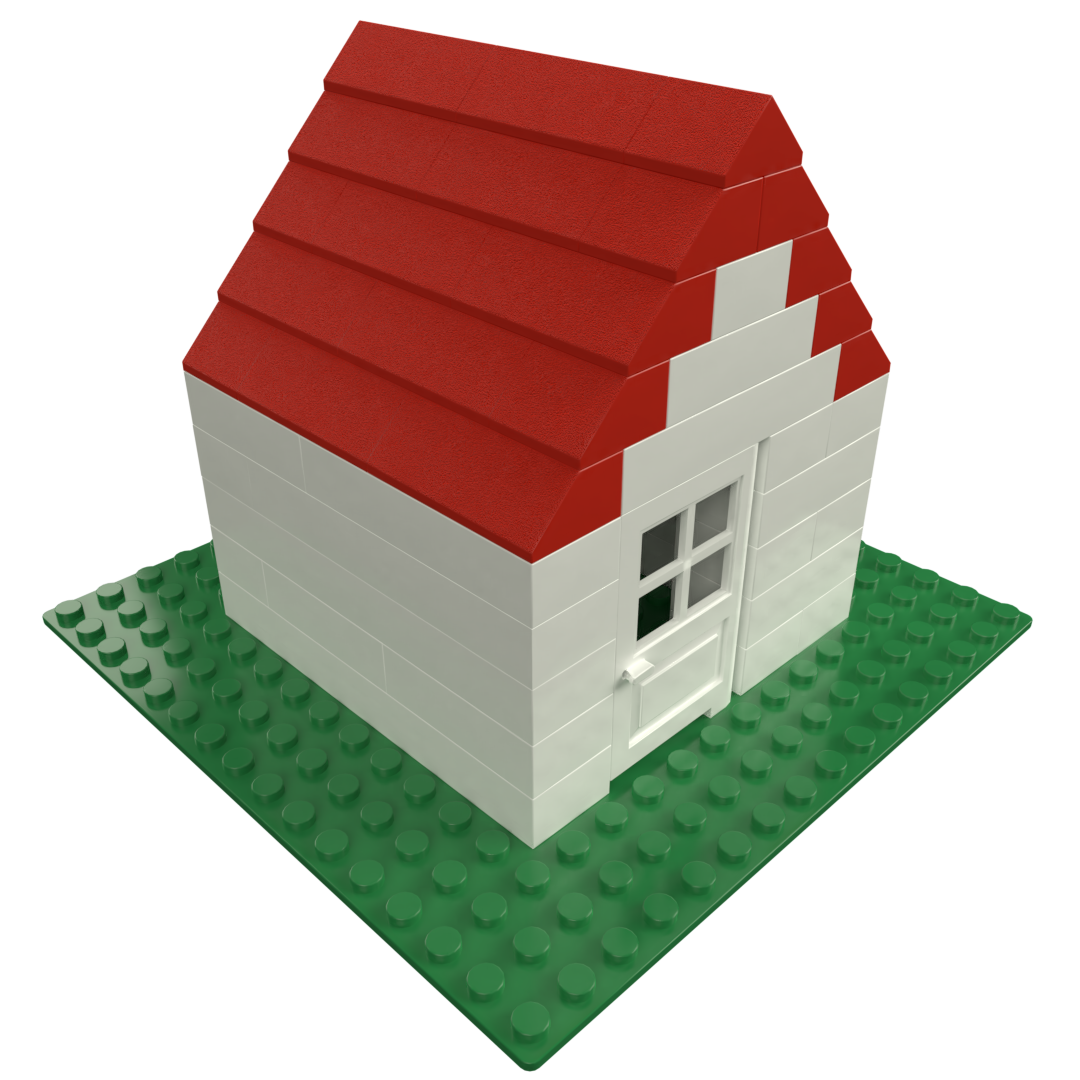
\includegraphics[width=\textwidth]{images/02_modelling_languages/lego_house.png}
    \end{column}\begin{column}{0.4\textwidth}
        \centering
        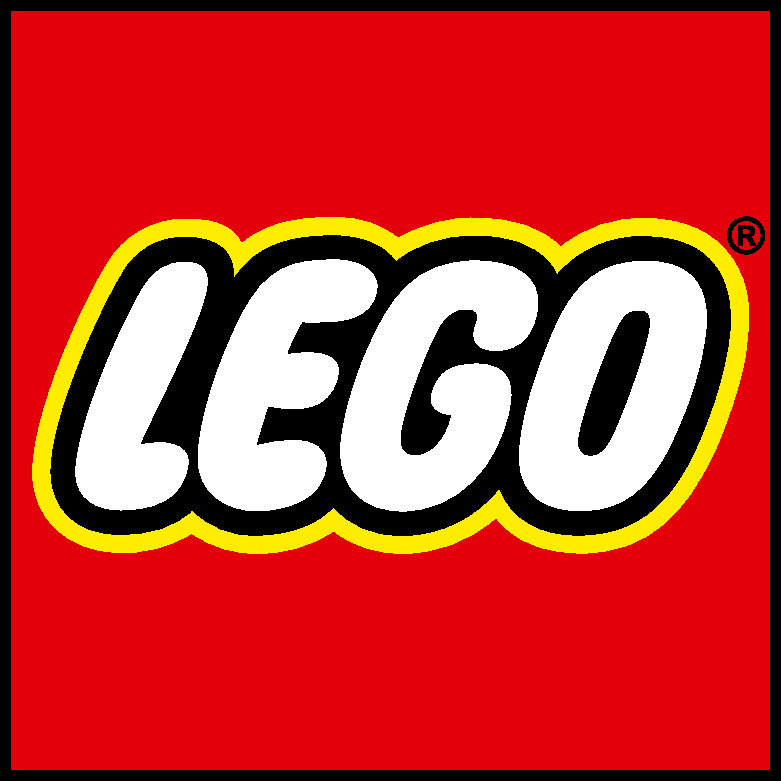
\includegraphics[width=0.5\textwidth]{images/02_modelling_languages/LEGO_logo.pdf}
        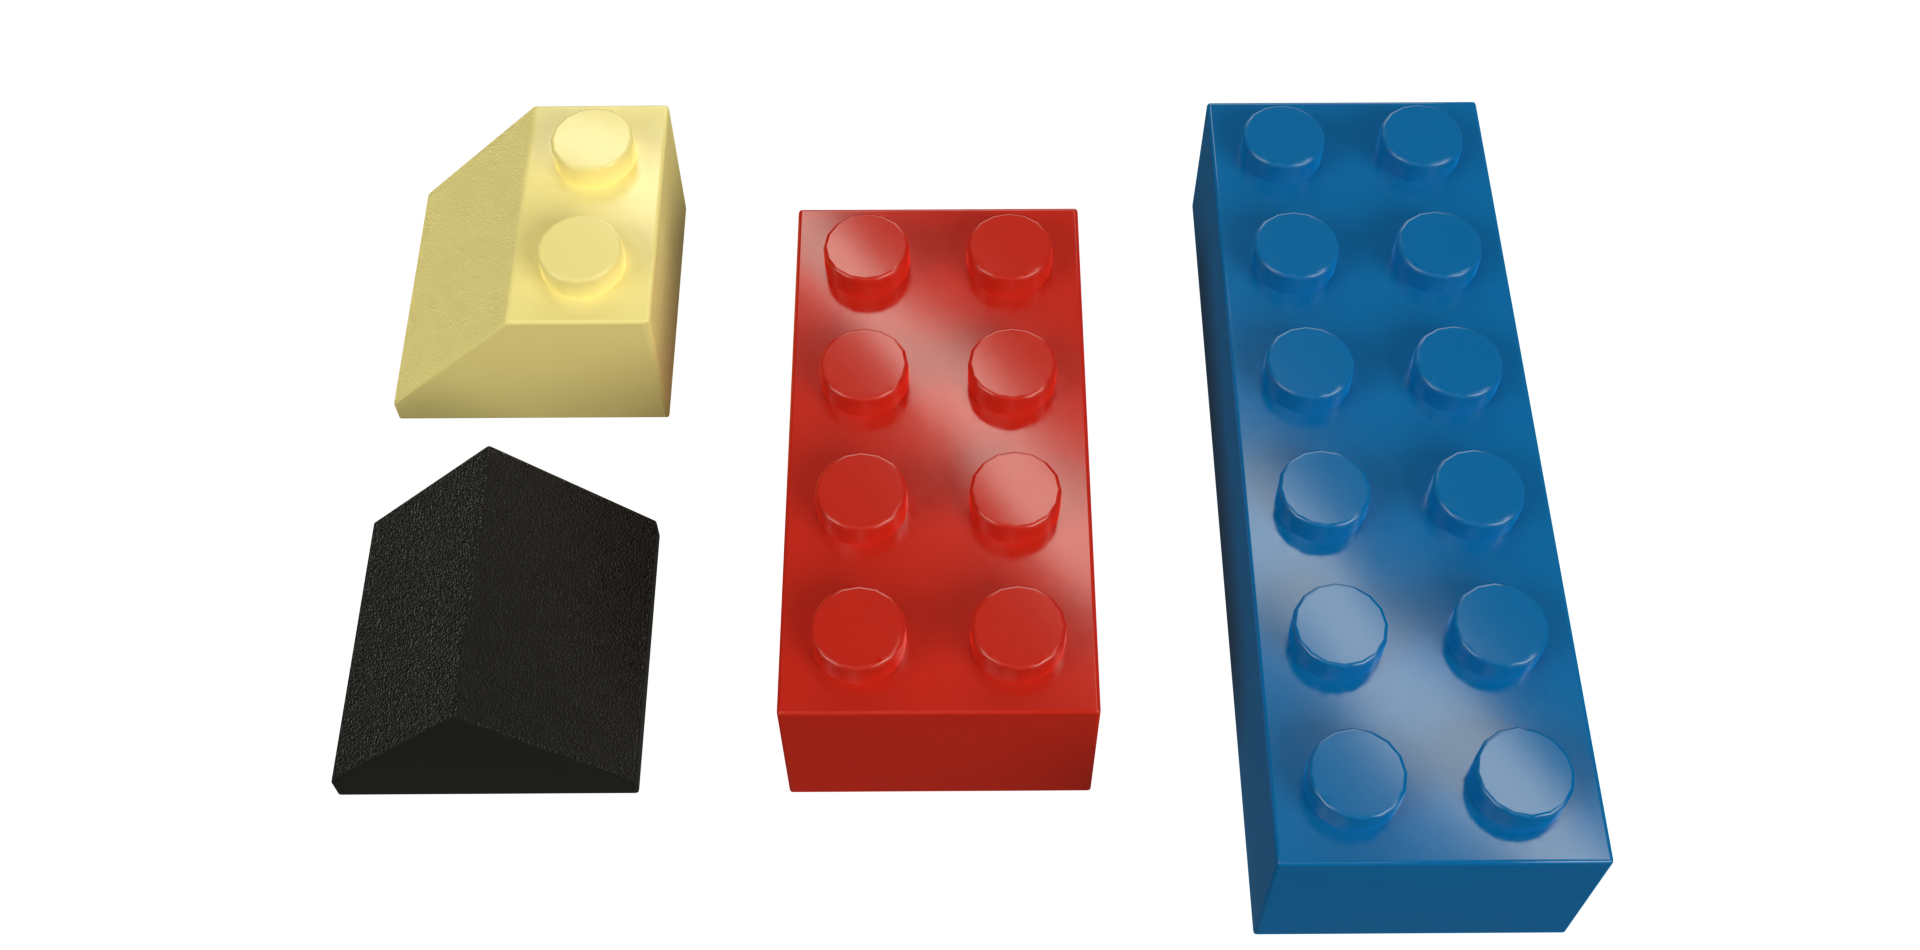
\includegraphics[width=\textwidth]{images/02_modelling_languages/lego_brick_examples.png}
    \end{column}
\end{columns}
\end{frame}

\note{
	\begin{itemize}
	    \item Explain what a modelling language is informally, ignore the definition.
	    \item Explain that you could think of Lego as a modelling language.
	\end{itemize}
}

\begin{frame}{Modelling languages}
    EMF/Ecore
    \begin{itemize}
        \item Eclipse Modelling Framework
        \item Modelling framework and code generation facility
        \item Modelling language rules enforced by metamodel Ecore
    \end{itemize}
    \pause
    GROOVE
    \begin{itemize}
        \item GRaphs for Object-Oriented VErification
        \item Software verification tool using graph grammars
        \item Modelling language rules based on graph grammars
    \end{itemize}
\end{frame}

\note{
	\begin{itemize}
	    \item Explain that within this thesis, we use software modelling languages.
	    \item Explain shortly what Ecore is
	    \item Explain shortly what GROOVE is
	\end{itemize}
}

\begin{frame}{Modelling languages}
    For Ecore, 2 different model types are considered:
    \begin{itemize}
        \item Type models, directly based on the Ecore metamodel
        \item Instance models, based on a type model
    \end{itemize}
    \pause
    For GROOVE, 2 different graph types are considered:
    \begin{itemize}
        \item Type graphs
        \item Instance graphs, based on a type graph
    \end{itemize}
\end{frame}

\note{
	\begin{itemize}
	    \item Explain that for Ecore, two different levels of models are considered, type models and instance models.
	    \begin{itemize}
	        \item Type models are best viewed as UML class diagrams
	        \item Instance models are instatiations of these diagrams.
	    \end{itemize}
	    \item Explain that for GROOVE, we have similar levels
	    \begin{itemize}
	        \item Type models will be transformed into type graphs, which are graphs that define a some structure of node types and edge types.
	        \item Instance models are transformed into instance graphs, which is an instantiation of the structure defined by the type graph.
	    \end{itemize}
	\end{itemize}
}

\begin{frame}{Ecore type model}
    \centering
    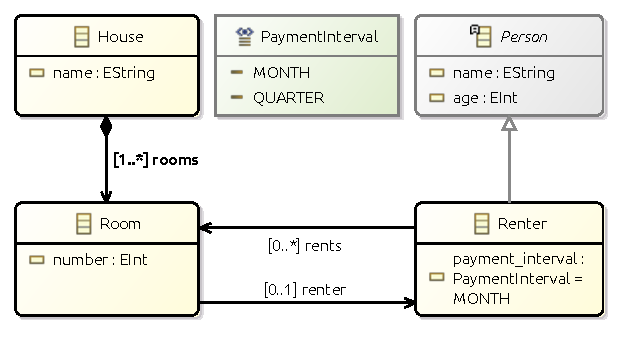
\includegraphics[width=0.9\textwidth,trim={0 0.45cm 0 0.25cm},clip]{images/02_modelling_languages/type_model_example.pdf}
\end{frame}

\begin{frame}{GROOVE type graph}
    \centering
    % To use this figure in your LaTeX document
% import the package groove/resources/groove2tikz.sty
%
\begin{tikzpicture}[scale=\tikzscale,name prefix=type-]
\node[type_node] (n0) at (0.560, -0.290) {\ml{\textbf{House}\\name: \textbf{string}}};
\node[type_node] (n1) at (0.600, -1.430) {\ml{\textbf{Room}\\number: \textbf{int}}};
\node[type_node] (n2) at (2.470, -1.435) {\ml{\textbf{Renter}}};
\node[type_node] (n3) at (2.470, -2.175) {\ml{\textit{\textbf{PaymentInterval}}}};
\node[type_node] (n4) at (1.170, -2.785) {\ml{\textbf{PaymentInterval\$MONTH}}};
\node[type_node] (n5) at (3.830, -2.785) {\ml{\textbf{PaymentInterval\$QUARTER}}};
\node[type_node] (n6) at (2.470, -0.375) {\ml{\textit{\textbf{Person}}\\age: \textbf{int}\\name: \textbf{string}}};

\path[subtype_edge](n2.north -| 2.470, -0.375) --  (n6) ;
\path[subtype_edge] (n4)  --  (n3) ;
\path[subtype_edge] (n5)  --  (n3) ;
\path[basic_edge](n2.west |- 0.600, -1.430) -- node[lab] {\ml{rents}} (n1) ;
\path[basic_edge, composite](n0.south -| 0.600, -1.430) -- node[lab] {\ml{rooms}} (n1) ;
\path[basic_edge](n2.south -| 2.470, -2.175) -- node[lab] {\ml{payment\_interval}} (n3) ;
\path[basic_edge](n1.east |- 2.470, -1.435) -- node[lab] {\ml{renter}} (n2) ;
\end{tikzpicture}

\end{frame}

\note{
	\begin{itemize}
	    \item Explain type model and type graph. Show that they have the same elements.
	    \item Explain that certain elements need to be encoded.
	\end{itemize}
}

\begin{frame}{Ecore instance model}
    \centering
    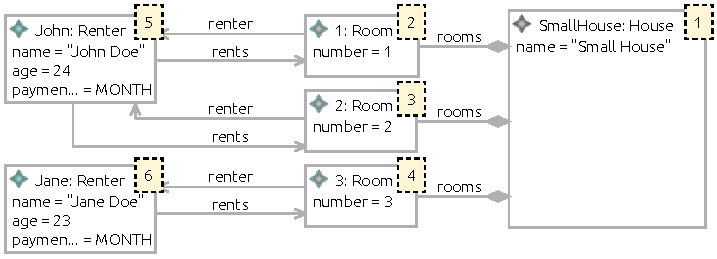
\includegraphics[]{images/02_modelling_languages/instance_model_example.pdf}
\end{frame}

\begin{frame}{GROOVE instance graph}
    \centering
    % To use this figure in your LaTeX document
% import the package groove/resources/groove2tikz.sty
%
\begin{tikzpicture}[scale=\tikzscale,name prefix=start-]
\node[basic_node] (n0) at (2.235, -0.335) {\ml{\uline{\textit{Renter1}} : \textbf{Renter}\\age = 24\\name = "J.A."}};
\node[basic_node] (n1) at (2.225, -2.305) {\ml{\uline{\textit{Renter2}} : \textbf{Renter}\\age = 23\\name = "M.S."}};
\node[basic_node] (n2) at (1.005, -1.345) {\ml{\textbf{PaymentInterval\$MONTH}}};
\node[basic_node] (n3) at (4.605, -0.330) {\ml{\uline{\textit{Longhorn}} : \textbf{Room}\\number = 1}};
\node[basic_node] (n4) at (4.585, -1.370) {\ml{\uline{\textit{Shorthorn}} : \textbf{Room}\\number = 2}};
\node[basic_node] (n5) at (4.595, -2.330) {\ml{\uline{\textit{onghornLay}} : \textbf{Room}\\number = 3}};
\node[basic_node] (n6) at (6.975, -1.380) {\ml{\uline{\textit{TwoRem}} : \textbf{House}\\name = "Small House"}};

\path[basic_edge] (n6)  -- node[lab] {\ml{rooms}} (n5) ;
\path[basic_edge](n6.west |- 4.585, -1.370) -- node[lab] {\ml{rooms}} (n4) ;
\path[basic_edge](n3.west |- 2.235, -0.235) -- node[lab] {\ml{renter}} (n0) ;
\path[basic_edge] (n4.west)  -- node[lab] {\ml{renter}} (n0) ;
\path[basic_edge](n5.west |- 2.225, -2.205) -- node[lab] {\ml{renter}} (n1) ;
\path[basic_edge] (n0)  -- node[lab] {\ml{payment\_interval}} (n2) ;
\path[basic_edge] (n6)  -- node[lab] {\ml{rooms}} (n3) ;
\path[basic_edge] (n0) -- node[lab] {\ml{rents}} (n3.west |- 4.605, -0.430) ;
\path[basic_edge] (n1)  -- node[lab] {\ml{payment\_interval}} (n2) ;
\path[basic_edge](n1) -- node[lab] {\ml{rents}} (n5.west |- 4.595, -2.430) ;
\path[basic_edge] (n0)  -- node[lab] {\ml{rents}} (n4.north) ;
\end{tikzpicture}

\end{frame}

\note{
	\begin{itemize}
	    \item Explain instance model and instance graph. Show that it are instantiations of their type counterparts.
	\end{itemize}
}